\cleardoublepage

\section{RISCV处理器瞬态执行漏洞挖掘背景}

\subsection{RISC-V指令集架构}

RISC-V 指令集架构(ISA)是一种开源的精简指令集架构\cite{riscv-isa-manual-all}。
它由一个基本的整数指令集和一组可选的指令集扩展组成。
标准扩展包含整数乘除法扩展(M)、内存原子操作扩展(A)、单精度浮点扩展(F)、双精度浮点扩展(D)和压缩指令扩展(C),等。
此外,控制和状态寄存器指令扩展(ZICSR)提供特权态管理功能, 而屏障指令扩展(ZIFENCEI)提供指令内存同步功能。\par

\begin{figure}[!h]
    \centering
    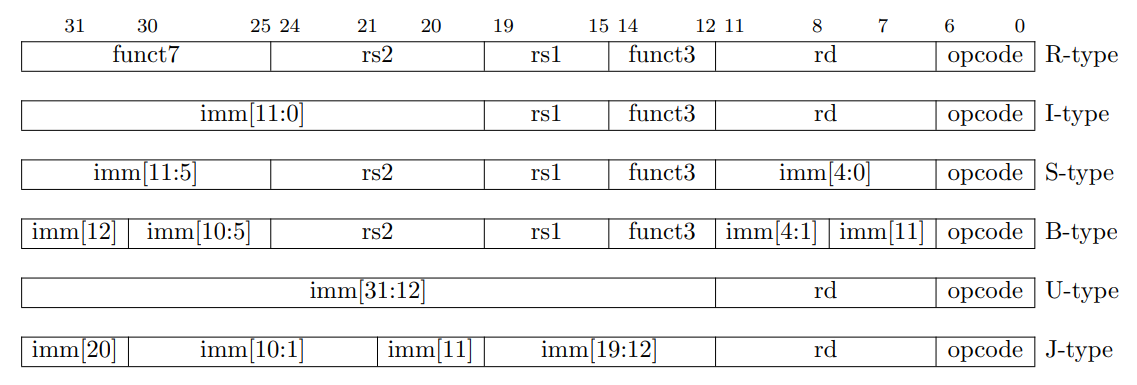
\includegraphics[width=\linewidth]{figure/proposal/riscv-base-instruct-format.png}
    \caption{RISCV基本指令格式}
    \label{review:base-inst}
\end{figure}
\begin{figure}[!h]
    \centering
    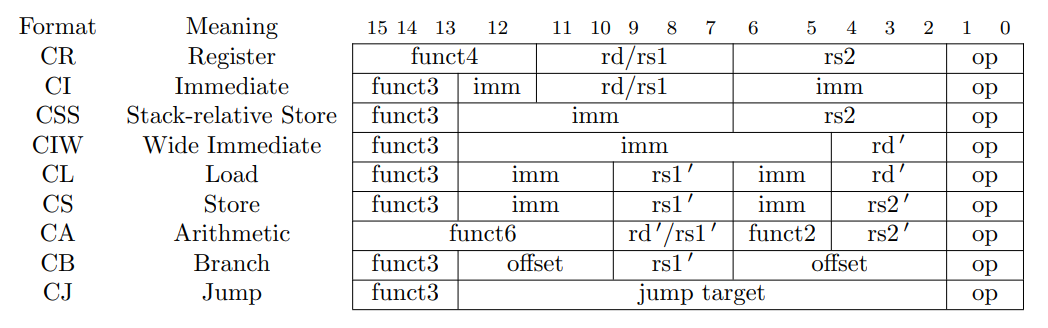
\includegraphics[width=\linewidth]{figure/proposal/riscv-compress-instruct-format.png}
    \caption{RISCV压缩指令格式}
    \label{review:compress-inst}
\end{figure}

RISC-V 指令分为 32 位常规指令(包含六种指令格式)和 16 位的压缩指令(包含九种指令格式)两种。 
图\ref{review:base-inst}和图\ref{review:compress-inst}显示了所有 15 种指令类型的格式,
每种指令由多个字段组成。32 位指令的指令格式由 opcode 字段决定,而 16 位指令的格式由 op 和 funct 字段同时决定。\par

指令字段可分为两类:\par

第一类是操作码相关字段,如 funct 和 opcode 字段。
opcode 字段和 op 字段的低 2 位用于确定指令的长度,而 funct 字段和 opcode 字段的其它位用于确定指令格式和功能。
通常,具有相似功能的指令有相同的 opcode 字段,并通过 funct 字段来区分具体功能。\par

第二类是操作数相关的字段,包括 imm,rs 和 rd 字段。
其中 rs 字段用于选择源寄存器,imm 字段用于表示立即数,rd 字段用于选择目的寄存器,即写回指令结果的寄存器。\par

\subsection{瞬态执行攻击}
瞬态执行漏洞是现代处理器的关键漏洞。
现代处理器为了追求高性能,广泛采用乱序执行和投机执行等技术提高硬件利用率。
由于异常延迟处理和推测错误等原因,部分指令会被错误执行,虽然其执行结果会在后续被撤销,
并不会影响处理器架构层执行结果的正确性,但仍可能引起处理器微架构的状态变化。
攻击者可以通过侧信道跟踪微架构的状态变化,进而恢复出处理器内部的机密信息,这种攻击方式称为瞬态执行攻击。\par

瞬态执行攻击过程可以分为如下三个阶段。\par

\textbf{触发瞬态执行窗口:}
通过操纵控制流和数据流,可以人为创造异常延迟处理或者推测错误等场景,触发瞬态执行窗口,从而临时性的绕过软硬件的安全权限检查。
例如 Meltdown 类型利用了延迟的权限检查,如延迟对页表条目中的标志位的检查\cite{horn2018meltdown},
或对浮点寄存器权限的检查\cite{stecklina1806lazyfp},暂时绕过硬件原语的安全权限检查,瞬态执行后续的代码;
而 Spectre 类型\cite{kocher2020spectre} 则通过毒害返回地址堆栈\cite{maisuradze2018ret2spec}、分支预测器等,
操纵控制流进入错误预测的跳转地址,从而暂时绕过软件的安全权限检查,瞬态执行错误预测地址之后的代码。\par

\textbf{访问秘密数据:}
在第一阶段触发瞬态执行窗口之后,处理器可以临时性的绕过软硬件的安全权限检查,执行没有安全权限的代码。
通过执行这些代码可以直接或者间接访问内存中的秘密数据,将秘密数据暂时从存储部件泄漏到寄存器中\cite{van2019ridl}\cite{van2021cacheout}。
这里可以直接访问秘密数据的地址,将内存、缓存、load buffer 中的秘密数据泄漏到寄存器中;
也可以访问低位对齐等相关的地址,将存储层次中的秘密数据泄漏到寄存器。

\textbf{使用侧信道泄露秘密数据:}
将秘密数据带入寄存器之后,通过微体系结构的微架构状态对秘密数据进行编码。
之后通过特殊的微架构跟踪技术,通过时间侧信道等侧信道,将编码在微架构状态中的秘密数据解码出来,从而实现秘密数据的侧信道泄露。
已知的瞬态执行漏洞往往通过缓存\cite{yarom2014flush+}、分支预测器\cite{evtyushkin2018branchscope}、
执行端口\cite{bhattacharyya2019smotherspectre}等微架构部件进行秘密数据的编码,
然后通过时间侧信道将编码在其中的信息泄露出来。
随着 cpu 复杂度的不断提高和瞬态攻击研究的不断推进,更多微架构状态和侧信道被用于瞬态攻击的执行。\par

\subsection{处理器 Fuzzing}

Fuzzing 一种自动化的测试技术,它会根据一定的规则自动或者半自动地生成随机数据,
然后输入到动态运行的被测程序入口,通过监控被测程序是否有异常情况发生(如系统崩溃,断言失败等)来发现存在的软件缺陷。
同时一些 Fuzzing 生成器会根据被测程序插桩的信息反馈,有指向性的对输入数据进行突变,
进一步提高异常触发的效率和提高程序测试的覆盖率。
随着处理器复杂程度的提高,传统的处理器验证方式效果开始不断受限,
研究人员转而将 Fuzzing 技术引入到处理器正确性验证领域 
\cite{bruns2022efficient}\cite{canakci2021directfuzz}\cite{hur2021difuzzrtl}。\par

处理器 Fuzzing 和软件 Fuzzing 一样也由三个阶段组成:\par

1.输入生成阶段:
模糊器使用种子生成指令流,并根据前一轮的覆盖范围对指令流进行突变,
如 DifuzzRTL\cite{hur2021difuzzrtl}使用静态分析技术生成指令,
而 Huzz\cite{kande2022thehuzz} 则使用最优权重优化算法进行突变。\par

2.硬件仿真阶段:
Fuzzing 工具使用硬件插桩技术来收集当前输入的覆盖率,现有的 Fuzzing 工具设计了多种覆盖度量,
诸如 mux 覆盖\cite{laeufer2018rfuzz}、控制寄存器覆盖\cite{hur2021difuzzrtl}和硬件行为覆盖\cite{kande2022thehuzz} 等。\par

3.状态验证阶段:
Fuzzing 工具提取 DUT 的架构状态,然后将其与参考模型(例如,ISA 模拟器)进行比较,其中不匹配的行为将被标记为 bug。\par

\par

\textbf{差分模糊测试:}
差分测试需要一种检测机制来检测错误或者说检测异常行为。
虽然一些简单的错误如内存损坏、段错误等很容易被检测器捕获,但那些难以定义明确异常行为的语义错误则很难被检测到。
因此,差分测试被用于识别语义相关的 bug,它通过比较具有相同功能和执行目标的多个程序的执行结果进行错误检测,
如果这些程序显示不同的输入-输出关系,则可以认定这是一个bug。\par

瞬态执行漏洞因其语义的复杂性,难以用简单的逻辑约束进行表征和检测,
而差分测试正好适用于语义相关 bug 的识别,故而也被广泛运用于瞬态执行漏洞的检测。
具体方法如下:将两个仅秘密数据部分不同的可执行程序交给两个同样的处理器进行执行,如果两者执行的时间存在差异,
则可以认为可以通过时间侧信道对秘密数据进行泄露。

\subsection{国内外相关工作}

瞬态指令漏洞的 Fuzzing 检测作为处理器 Fuzzing 的变体,可以类似的分为输入生成阶段、测试执行阶段和漏洞检测阶段三部分。
本章节将从这三个方面分别进行研究方向和研究进展的介绍。

\subsubsection{输入生成}
输入生成阶段负责生成尝试触发瞬态执行漏洞的测试程序。\
早期的硬件 Fuzzing 工具如 DifuzzRTL\cite{hur2021difuzzrtl}、
TheHuzz\cite{kande2022thehuzz}等基本采用纯随机的方式进行测试指令的生成,
处理器漏洞挖掘效率相对较低。为了进一步提高测试程序的质量,Razzle\cite{razzle}、
Cascade\cite{soltcascade}等工具会对程序的控制流进行约束,以此提高程序执行的覆盖率;
SpecDoctor\cite{hur2022specdoctor}等工作对指令的数据流进行了约束,
通过提高相邻指令的数据依赖,提高其在处理器微架构执行时的难度。\par

为了充分利用瞬态执行漏洞的语义特点,一些测试程序生成工具采用基于模板突变的方法,
试图高效的产生瞬态执行漏洞的变体。如Transynther\cite{moghimi2020medusa}是专注于 MDS 变体生成的工具,
它使用已知的MDS构建块和微代码进行组合,来构造新的 MDS 泄漏,
而SpeechMiner \cite{xiao2019speechminer}则专注于 Meltdown 变体的生成。
但这种方法可能会导致漏洞同质化,缺乏挖掘全新漏洞的能力。\par

\subsubsection{测试执行}

测试执行阶段负责让后端处理器执行前端生成的测试程序,尝试在执行中触发瞬态执行漏洞。
早期的工作会直接使用真实的处理器硬件执行测试程序,但是随着RTL漏洞检测重要性的提高,
基于RTL仿真的瞬态漏洞测试执行工作,如IntroSpectre\cite{ghaniyoun2021introspectre}、
SpecDoctor\cite{hur2022specdoctor}等开始兴起。
Verilator\cite{snyder2013verilator}等开源工具为RTL仿真提供了条件,
且在仿真的场景下还可以进行硬件插桩,便于后续阶段的漏洞检测。\par

但为了提高测试执行的效率,一些工作如Revixor\cite{oleksenko2022revizor}、
Scam-V\cite{nemati2020validation}、
Speculation at Fault\cite{hofmann2023speculation}等会对处理器硬件建立形式化模型,
然后基于形式化模型进行测试执行,其中Revixor\cite{oleksenko2022revizor}支持 x86 指令,
Scam-V\cite{hofmann2023speculation}支持 arm 指令,
Speculation at Fault\cite{hofmann2023speculation}则是对Revixor\cite{oleksenko2022revizor}
在异常相关类型漏洞上的一个补充。此外基于模型的测试方式也可以对模型直接进行瞬态执行漏洞的静态分析,
如UPEC\cite{fadiheh2020formal}根据开源RTL手动建立有界模型,然后利用静态分析的技术寻找瞬态漏洞。

\subsubsection{漏洞检测}

漏洞检测阶段负责对测试执行的结果进行分析,进而判断是否触发了瞬态执行漏洞。
差分测试是广泛使用的瞬态执行漏洞检测的方法,Revixor\cite{oleksenko2022revizor}、
Speculation at Fault\cite{hofmann2023speculation}等工作都使用差分测试进行瞬态执行漏洞检测,
SpecDoctor\cite{hur2022specdoctor}更是在两个不同的阶段分别运用了差分测试。\par

此外还可以用基于约束的方法进行瞬态执行漏洞的检测,如Transynther\cite{moghimi2020medusa}、
IntroSpectre\cite{ghaniyoun2021introspectre}通过检查缓冲区执行前后的变化进行漏洞检查,
SpeechMiner\cite{xiao2019speechminer}通过测量竞争条件判断漏洞的可用性。\par

差分测试和约束判断的漏洞检测方法有时还需要硬件插桩的辅助。
如果拥有 RTL 的源码,就可以通过 RTL 硬件插桩的方法为检测程序得到处理器内部的状态信息和事件信息,
甚至可以在处理器内存内嵌约束判断的电路逻辑,在测试执行的同时直接进行漏洞约束的判断。

\section{研究挑战}

在生成瞬态执行漏洞的测试程序的时候,生成框架会遇到三个重要挑战。
首先,在指令生成层面,
生成框架生成的指令需要生成满足特定条件的操作数和指令间依赖,
以满足特定的数据流和控制流约束;
其次,为了高效地生成能触发瞬态窗口的代码,
生成框架需要有意识地为瞬态窗口触发指令设计和排布训练代码;
最后,为了生成有效的测试程序,生成框架需要将零散生成的瞬态执行漏洞各阶段
的代码有效组合起来,并且删除一些冗余的代码,提取出精简的测试程序。

\subsection{带约束的指令生成}
\textbf{约束指令操作数}。
为了触发瞬态执行漏洞,生成框架生成的指令需要能执行特定的操作。
例如为了可以泄露秘密数据或者触发内存访问异常,
访存指令计算得到的操作数需要落在特殊的内存地址范围内;
为了让控制流指令可以跳转到预设的地址,跳转指令计算得到的跳转地址需要等于预设的地址、
分支指令操作数的值要满足对应的比较规则等。
为了确保指令在执行时可以得到满足要求的操作数,从而实现特殊的语义行为(如跳到特殊地址、访问特殊内存等),
在生成指令时需要对指令立即数字段、数据段值、指令组合等进行约束处理。\par

\textbf{约束指令字段}。
为了触发一些预设的特殊场景,生成框架也需要对生成指令的字段进行约束。
例如为了增加指令间的数据流依赖,触发更复杂的流水线执行情况,需要对指令间的 rs、rd 等字段进行约束;
为了可以跳转到特定的地址、访问特殊的内存,需要对指令和数据的 label 等进行约束。\par

\subsection{瞬态窗口训练的生成}
\textbf{训练代码的生成}。
Spectre 等瞬态执行漏洞指出,触发瞬态窗口除了需要触发瞬态窗口的 trigger 指令(如 Spectre 的控制流指令、
Meltdown 的内存访问指令等),还需要有指令序列对 trigger 相关的微架构部件进行微架构状态的训练。
但是以往的工作如DifuzzRTL\cite{hur2021difuzzrtl}、TheHuzz\cite{kande2022thehuzz}、
SpecDoctor\cite{hur2022specdoctor}都是用随机代码生成的方式进行瞬态窗口触发代码的生成,
并没有有针对性地生成训练代码,这导致了瞬态窗口的生成效率低下。
故而生成器需要能根据 trigger 指令,有针对性地生成用于训练的指令序列,进而提高瞬态窗口触发的可能性。\par

\textbf{地址敏感的代码排布}。
指令序列对 trigger 的训练效果是地址敏感的。在多数情况下,训练指令只有在特殊的地址上才可以有效训练 trigger 指令对应的微架构状态。
例如对于 BOOM 处理器\cite{celio2017boomv2}的 branch 指令,
低地址对齐的控制流指令可以对该 trigger 对应的分支预测器表项进行有效训练,
从而将 branch 指令涉及的微架构调整到位。
为此,生成框架在生成训练代码的时候需要寻找合适的指令排布位置,
从而提高训练的成功率。 \par

\subsection{完整程序的生成}

\textbf{程序的组合}。
已知完整的瞬态执行漏洞程序由触发瞬态窗口、访问秘密数据、侧信道泄露秘密数据三部分代码组成,
因此生成框架需要将生成得到的三部分代码进行有效的地址排布和控制流约束,确保三部分代码能够依次执行,
从而组成完整有效的瞬态漏洞程序。这要求我们通过总结分析三部分代码内部的指令排布和代码间的指令排布的关系,
设计出通用的代码组装模版,在确保瞬态漏洞程序有效运行的同时,尽可能多地覆盖各类瞬态漏洞场景。\par

\textbf{程序的精简}。
生成器得到的瞬态执行漏洞程序不可避免地包含了许多对瞬态执行攻击没有帮助的指令,
这些指令会增加程序模拟执行、漏洞检测时的时间开销,并且也会对后续定位程序中的漏洞带来负担。
因此生成框架需要使用合适的算法精简掉各部分冗余的指令,从而得到简短的高质量瞬态漏洞程序。\par

\section{测试程序生成框架的设计}

本生成框架是一种针对 RISCV 处理器 RTL 的、用于瞬态漏洞查找的测试程序生成框架。
对于给定的 RISCV 处理器 RTL,该生成框架可以根据瞬态执行漏洞各阶段的程序特点,
高效地生成瞬态执行漏洞测试程序,寻找发动瞬态执行攻击的具体 PoC,进而准确的复现漏洞。 \par

\subsection{生成框架概述}

为了高效地生成有效的瞬态执行攻击程序,我们的生成框架分两个阶段依次进行测试程序的生成。
在阶段1中,生成框架生成触发瞬态窗口的指令序列,并在处理器 RTL 上检验该部分指令的有效性;
阶段2在阶段1成功的基础上,生成访问秘密数据和利用侧信道传递秘密数据的指令序列,
如果该指令序列在处理器上,通过差分测试发现存在瞬态执行攻击行为,即可得到能有效执行的完整 PoC。\par

\subsection{阶段1:触发瞬态窗口}

不同于 SpecDoctor 先生成能触发瞬态窗口的随机指令序列,再确定 trigger 指令和瞬态窗口位置;
我们的生成框架预先确定待触发的瞬态窗口和触发该瞬态窗口的 trigger 指令,再为 trigger 指令生成协同工作
的训练代码和其他代码。之后该测试程序会在 vcs 或者 verilator 生成的处理器 RTL 上模拟执行,
检查预设的瞬态窗口是否触发。如果触发成功,生成框架会删去冗余的训练指令,然后进入阶段2生成后续指令。\par

\subsubsection{瞬态窗口触发代码的生成与排布}

为了实现触发瞬态窗口的目的,生成框架会生成如下配合工作的的代码块:\par

\textbf{全局初始化块(init块):}
init 块负责在程序执行伊始为所有特权寄存器赋初值,然后执行后续的瞬态窗口触发代码代码。\par
\textbf{退出块(exit块):}
exit 块负责 RTL 仿真程序的结束,当瞬态窗口测试代码执行完毕后进入 exit 块退出程序。\par
\textbf{后续初始化块(load\_init块):}
load\_init 块负责为后续所有被执行的块所使用的通用寄存器和浮点寄存器提供随机的初值或者传递指定的参数。\par
\textbf{延迟块(delay块):}
delay 块在 load\_init 块初始化之后执行,它由一系列强数据流依赖的多周期指令组成,用于延迟得到操作数的计算结果。\par
\textbf{触发块(trigger块):}
trigger 块负责触发瞬态窗口,紧接着 delay 块开始执行。为了延迟得到 trigger 指令的执行结果,迫使处理器执行预测执行,trigger 指令的操作数需要依赖于 delay 块的计算结果。
此外,为了可以让 trigger 指令可以访问特殊的地址触发异常、或者跳转到非瞬态窗口的地址,生成框架会对 trigger 指令的操作数值进行约束,
确保地址访问或者地址跳转符合预期。\par
\textbf{瞬态窗口块(trans块):}
trans 块包含一个确保可以侧信道泄露秘密数据的默认指令序列,用于填充预设的待触发的瞬态窗口区域,如果该部分的代码被瞬态执行,则预示着瞬态窗口被触发成功,该代码块退出到 exit 块。\par
\textbf{返回块(return块):}
return 块作为控制流指令类型的 trigger 块正确执行后跳转到的无害代码,该代码退出到 exit 块。\par
\textbf{空操作块(nop 块):}
nop 块被放置在 load\_init\_train 块和 delay 块之间,用于排空流水线,防止 delay 块、trigger 块在执行的过程中被 load\_init 块的内存访问指令的执行所影响。\par
\textbf{异常块(trap块):}
trap 块作为异常触发类型的 trigger 块正确执行后跳转到的无害代码,该代码退出到 exit 块。\par

其中 init 块、return 块、exit 块、trap 块是因为测试框架需要所涉及的,因此称为功能块(function 块);
load\_init 块、nop 块、delay 块、trigger 块用于瞬态窗口的触发,因此称为触发块(trigger 块);
trans 块暂时填充阶段二用于秘密数据泄露部分的代码的位置,因此属于泄露块(leak 块)。
根据瞬态漏洞触发的场景不同,生成框架用四种方式将上述代码块组织起来,如图\ref{paper:trigger-dist-situation}所示:\par

\textbf{场景一:} trigger 块的 trigger 指令是控制流指令,例如 branch、jmp 等,
预设的瞬态窗口紧接着 trigger 块排布,而 trigger 的跳转目标位于 trans 块之后的 return 块位置。
当程序正确执行时,trigger 的跳转指令会发生跳转进入 return 块然后进入 exit 块退出程序;
当程序前端预测部件预测错误,认为 trigger 指令不发生跳转或者跳转地址是紧挨着 trigger 块下一条指令时,
控制流会临时进入 trans 块进行瞬态执行。该情况可以囊括 spectre 的部分场景。\par

\textbf{场景二:} trigger 块的 trigger 指令是控制流指令(例如 branch、jmp 等),
或者不触发异常的顺序执行指令(例如 add、mul 等),
预设的瞬态窗口和 trigger 块不相邻,而 trigger 不发生跳转或者跳转目标紧接着 trigger 块。
此时可以让 return 块紧挨着 trigger 块排布,而 trans 块位于 return 块之后。
当程序正确执行时,trigger 的指令会进入 return 块然后进入 exit 块退出程序;
当程序前端预测部件预测错误,认为 trigger 指令发生跳转且跳转地址位于 trans 内部时,
控制流会临时进入 trans 块进行瞬态执行。该情况可以囊括 spectre 的部分场景。\par

\begin{figure}[!h]
    \centering
    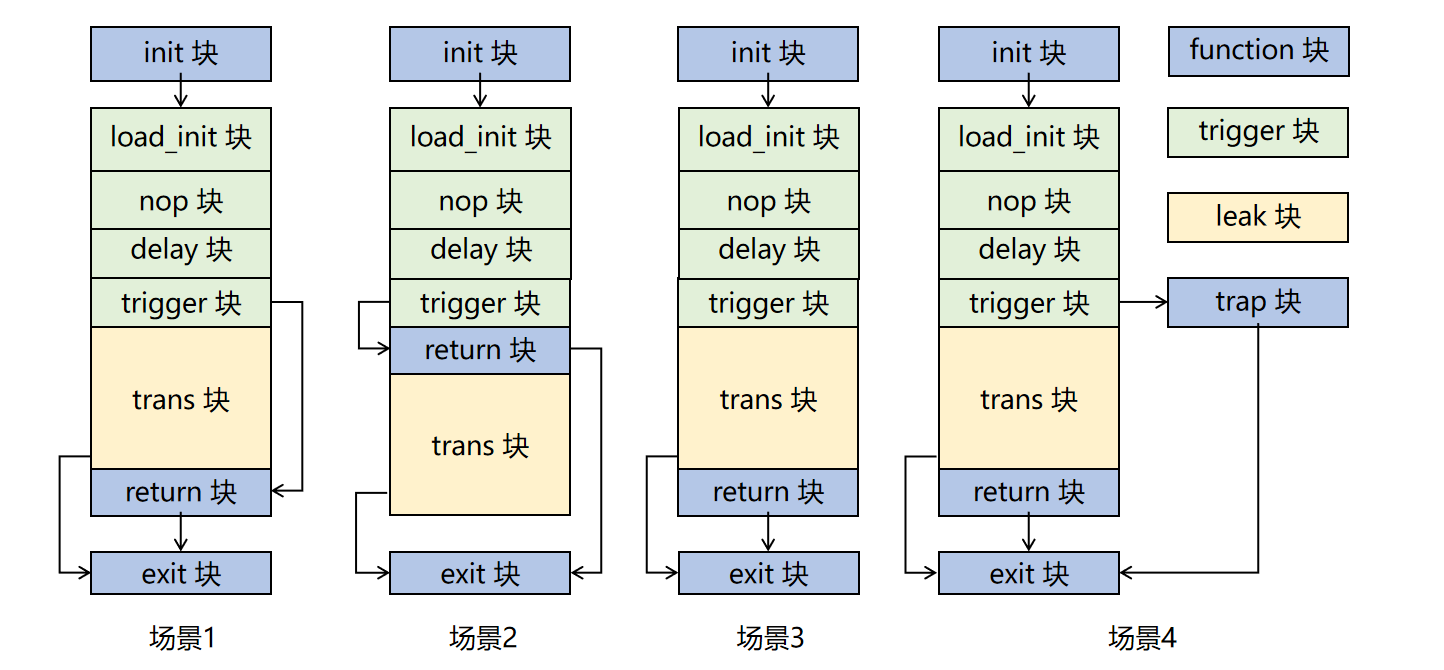
\includegraphics[width=\linewidth]{/mnt/d/txt/zjuthesis/figure/paper/arrange-stage1-situation.png}
    \caption{瞬态窗口触发代码块布局场景}
    \label{paper:trigger-dist-situation}
\end{figure}

\textbf{场景三:} trigger 块的 trigger 指令是 store 指令且修改 trans 块内部对秘密数据访问的地址时,
预设的瞬态窗口紧接着 trigger 块排布。当程序正确执行时,控制流进入了 trans 块,但是因为
秘密数据访问的地址被修改,使得秘密数据没有发生泄漏,之后进入 exit 块退出程序。
但是如果存在内存访问预测错误的情况,则会触发瞬态窗口,导致 trans 块会暂时用原先的秘密数据访问地址泄露秘密数据。
该情况可以囊括 spectre-v4 的场景。\par

\textbf{场景四:} trigger 块的 trigger 指令是触发异常的指令(例如 ecall、load、store 等),
预设的瞬态窗口紧接着 trigger 块排布。当程序正确执行时,
trigger 的指令触发异常进入 trap 块,然后进入 exit 块退出程序;
如果存在异常延时检查等情况,则 trigger 块后续的 trans 块的指令会继续被顺序执行,触发瞬态窗口。
该情况可以囊括 meltdown 的部分场景。\par

对上述场景适当合并和花间之后,代码的执行和排布顺序如图\ref{paper:trigger-dist}所示,首先执行 init 块,然后顺序排布和执行 load\_init 块、nop块、delay 块、trigger 块。
根据 trigger 指令的指令类别,决定后续排布的 return 块和 trans 块的顺序。trap 块位于其他位置,在异常发生的时候进入。
最后 return 块、trans 块、trap 块都会跳转进入 exit 块结束硬件模拟程序。这里的 load\_init 块、delay 块、trigger 块、nop 块
trans 块、return 块组成了一个完整的指令组合,我们称之为 victim group。\par

\begin{figure}[!h]
    \centering
    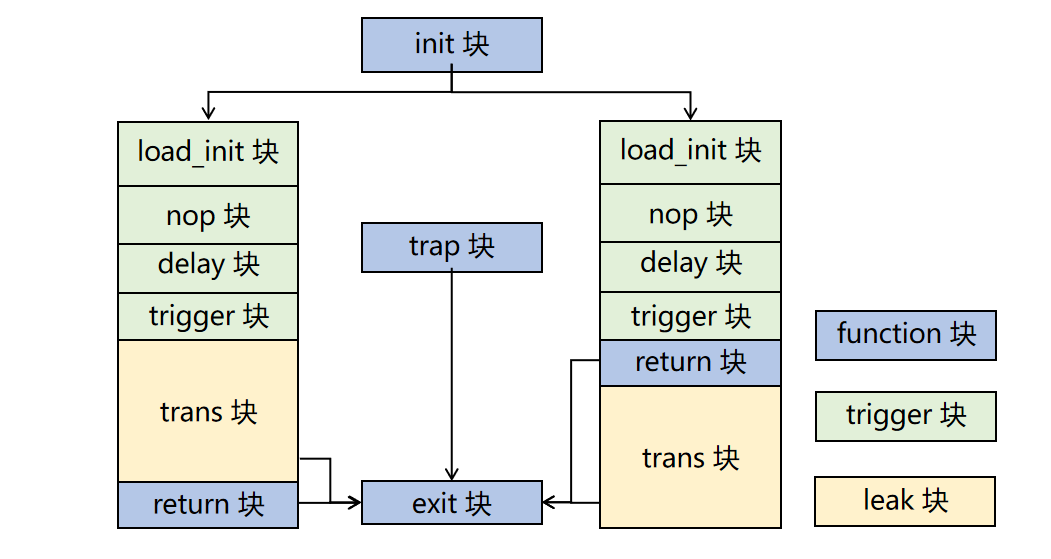
\includegraphics[width=\linewidth]{figure/paper/arrange-stage1.png}
    \caption{瞬态窗口触发代码块布局}
    \label{paper:trigger-dist}
\end{figure}

\subsubsection{训练代码的生成和排布}

为了 trigger 块的 trigger 指令可以更有效地触发瞬态窗口,生成框架需要生成额外的 train 指令对 trigger 指令进行训练,
因此生成框架在之前的基础上引入了用于训练的 train 块。train 块可以由一条或者多条任意类型的指令随机组合得到,
对于 train 块中的控制流指令和内存访问指令,生成框架对跳转地址和访问地址做额外约束,确保程序能正确执行。

考虑到 trigger 指令相关部件的微结构状态训练是地址敏感的,
因此 train 块布局的地址最好有和 trigger 的地址相关,如虚拟地址、甚至物理地址相同或者地址低位对齐等。
为了达到最高效的训练效果,也为了对物理地址空间和虚拟地址空间做最小的改动,
硬件额外扩展了一种 memory swap 的物理内存切换机制,可以硬件中对物理地址对应的内存单元直接进行切换,
从而确保 train 块和 trigger 块可以先后在同一物理地址执行,进而提高 train 块训练成功的概率。

为了实现充分多种类的训练功能,生成框架将会生成如下代码块:\par

\textbf{训练初始化块(load\_init\_train 块):}
load\_init\_train 块用于初始化 train 块需要的通用寄存器和浮点寄存器,提供随机值或者满足约束条件的特殊值,
该部分代码和 victim group 的 load\_init 块共享物理地址空间。\par

\textbf{训练块(train 块):}
train 块用于对 trigger 块的 trigger 指令设计的微架构状态进行调整,
该部分代码和 victim group 的 trigger 块共享物理地址空间

\textbf{空操作块(nop 块):}
nop 块被放置在 load\_init\_train 块和 train 块之间,
用于填充 train 块和 load\_init\_train 块之间的部分。\par

\textbf{返回块(return 块):}
同触发瞬态窗口的 return 块,用于作为 train 块中跳转指令的可选跳转目标,
和 victim group 的 return 块共享物理地址。\par

\textbf{空返回块(nop\_return 块):}
nop\_return 块用于填充 victim group 的 trans 块的位置,用于作为 train 块中跳转指令的可选跳转目标。\par

对于已生成的 victim group 指令序列,生成框架会生成对应地址布局的训练代码。这部分训练代码由上述的
load\_init\_train 块、nop 块、train 块、nop\_return 块、return 块组合而成,我们称之为 train group。
因为 train group 的 load\_init\_train 块、train 块的长度和 victim group 的 load\_init 块、trigger 块的长度
存在差异,为了确保它们的起始地址或者结束地址可以对齐,需要对 nop 块的长度进行调整。\par

有时候一个 train group 并不能有效训练 victim group,因此生成框架会依概率为 victim group
生成一系列 train group,依次执行,来提高成功训练 trigger 指令的可能性。
如图\ref{paper:memory-switch},当执行测试程序时,
首先执行第一个 train group 的指令序列,然后返回到物理内存切换的指令部分,
执行物理内存切换,物理内存的指令切换为下一个 train group 继续训练,直到最后切换为
被训练的 victim group 开始尝试触发瞬态窗口。\par

\begin{figure}[!h]
    \centering
    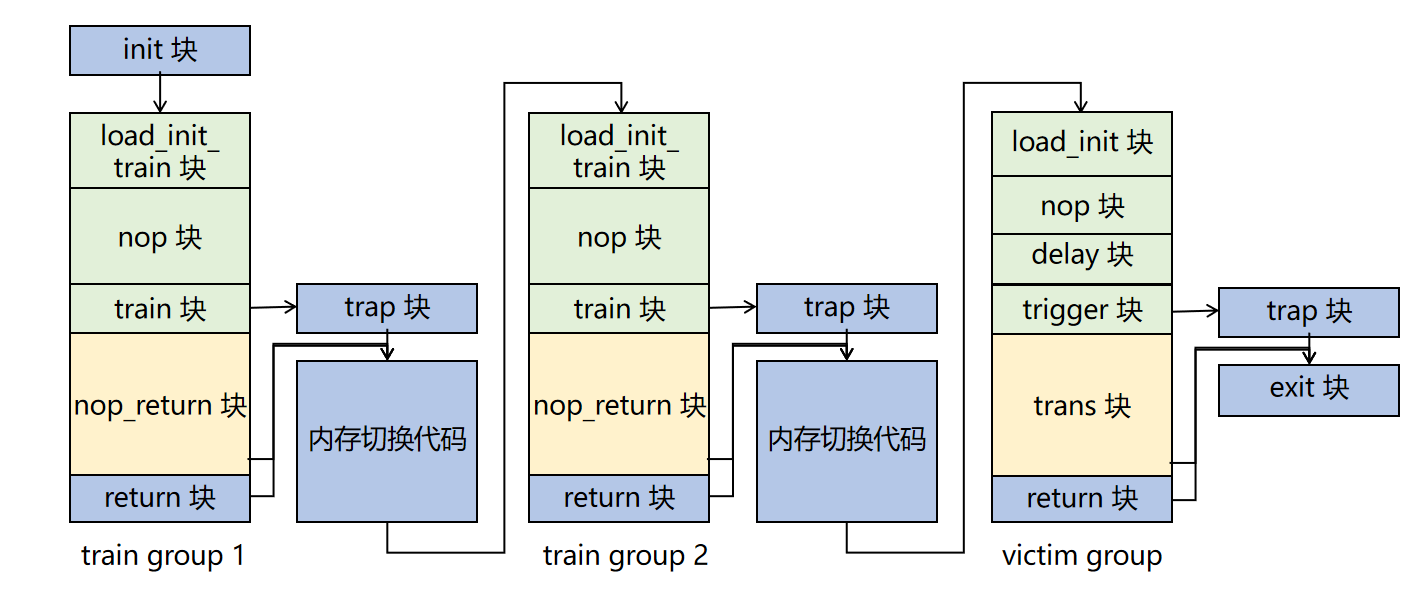
\includegraphics[width=\linewidth]{figure/paper/group-switch.png}
    \caption{代码组内存切换}
    \label{paper:memory-switch}
\end{figure}

\subsubsection{瞬态窗口触发检验}

为了判断阶段一生成的代码能否有效执行,生成框架生成的测试程序
需要在 vcs 或者 verilator 编译生成的处理器 RTL 上模拟执行,
检测是否触发了瞬态窗口,也即是否执行了 victim group 的 trans 块的代码。\par

为此生成程序预留了一组\textbf{slti zero, zero, imm}的指令作为 label 指令,用于标志特殊的指令事件的发生。
并会在 trans 块内部生成特殊的 label 指令 INFO\_TEXE\_START,表示瞬态执行窗口的开始。
之后我们对处理器的 rob 模块进行插桩,如果发现 label 指令进入 rob 和从 rob 中提交,就保存对应的 log 到指定文件。
如果 INFO\_TEXT\_START 指令进入 rob 的次数多于从 rob 中提交的次数,就说明 INFO\_TEXT\_START 在瞬态窗口中被执行了,
也即测试程序可以成功触发瞬态窗口,阶段一代码生成成功。

\subsubsection{测试程序的简化}

在为 victim group 生成 train group 序列的时候,测试框架为了确保 trigger 指令被有效训练,
可能会生成过饱和的 train group 序列。其中有部分 train group 可能是无效的,或者冗余的。
为了减轻后续阶段二执行 train group 的开销,也为了更好的定位训练 trigger 指令的有效 train 片段,
生成框架需要能删去多余的 train group 代码。\par

生成框架使用如下的算法\ref{alg:TS}进行 train group 的简化。该算法尝试删去 train group 序列中的一个 train group,
然后重新执行处理器模拟执行,如果仍然可以触发瞬态窗口,确认删去该 train group,然后尝试删除下一个 train group。
如果尝试删除所有的 train group 之后都无法出发瞬态窗口,则化简结束,得到局部最优的 train group 序列。\par

\begin{algorithm}[!h]
    \caption{Train Simplificaiton}
    \label{alg:TS}
    \renewcommand{\algorithmicrequire}{\textbf{Input:}}
    \renewcommand{\algorithmicensure}{\textbf{Output:}}
    
    \begin{algorithmic}[1]
        \REQUIRE train group list $train\_list$, vicitm group $victim$  %%input
        \ENSURE train group list after simplificaiton $new\_train\_list$    %%output
        \STATE $new\_train\_list \Leftarrow train\_list$
        \FOR{each $i \in [1, len(train\_list)]$}
            \FOR{each $j \in [1, len(new\_train\_list)$]}
                \STATE $tmp\_train\_list \Leftarrow new\_train\_list with new\_train\_list(i)$
                \IF{$trigger_test(tmp\_train\_list, victim) == True$}
                    \STATE $new\_train\_list \Leftarrow tmp\_train\_list$
                    \textbf{break}
                \ENDIF
            \ENDFOR
        \ENDFOR

        \RETURN $new\_train\_list$
    \end{algorithmic}
\end{algorithm}

\subsection{阶段2:访问和泄露秘密数据}

在阶段1得到的触发瞬态窗口代码的基础上,生成框架继续生成访问秘密数据和利用侧信道传递秘密数据的代码,
并通过处理器差分测试检测生成的测试程序能否最终触发瞬态执行攻击。
如果测试存在执行时间的差异,该测试程序即为完整的瞬态执行攻击的 PoC。

\subsubsection{访问秘密数据代码的生成与排布}

为了实现访问秘密数据的目的,生成框架会生成如下的代码块:\par

\textbf{秘密数据访问块(access\_secret 块):}
access\_secret 块的代码会生成待泄露的 secret 数据的地址,然后用 load 指令访问该内存,
将 secret 数据读取到寄存器中。生成的地址可以和秘密数据地址完全相同,也可以只是和秘密数据地址低位对齐的,
以尝试挖掘处理器潜在的 MDS 内存地址匹配漏洞。因为访问秘密数据的过程只能在瞬态执行的过程中进行,
因此 access\_secert 块的代码需要被布局在 trans 块的内部。\par

\textbf{秘密数据迁移块(migrate\_secret块):}
migrate\_secret 块负责转移 secret 数据在分层存储结构中的位置。处理器内存采用load缓冲区、cache、memory
的多层次存储结构,access\_secret 块的不同数据访问方式对不同深度的存储单元的访问能力是不同的,
因此生成框架需要产生秘密数据迁移的代码,将秘密数据迁移到合适的存储深度,提高 access\_secret 块
成功访问秘密数据的能力。migrate\_secret 仅使用其他块没有使用的寄存器进行操作,因此不会影响其他寄存器的执行结果。\par

如图\ref{paper:access-secret},
这两部分代码在阶段2会被组装进入 victim group。对于 access\_secret 块,
因为访问秘密数据的过程只能在瞬态执行的过程中进行,
因此 access\_secert 块的代码需要被布局在 trans 块的内部;
而对于 migrate\_secret 块,这部分代码虽然可以在瞬态窗口外部被执行,
但是在执行了 migrate\_secret 块的指令之后应该尽可能的避免内存访问指令的执行,
以防破坏 secret 在内存结构中的位置,因此这部分代码被放置在 load\_init 块之后,delay 块之前。
故而阶段2首先会根据随机配置,生成 access\_secret 块和 secret\_migrate 块,
并将原先的 victim group 调整为如图的布局。\par

当 victim group 的代码被执行时,程序在执行完 load\_init 块的寄存器初始化之后,
就会执行 secret\_migrate 块的代码将秘密数据迁移到处理器存储结构的合适位置,然后执行后续代码出发瞬态窗口。
瞬态窗口被触发之后,access\_secret 块被执行,试图将 secret\_migrate 块迁移之后的秘密数据
从存储层次结构读取到寄存器中。\par

\begin{figure}[!h]
    \centering
    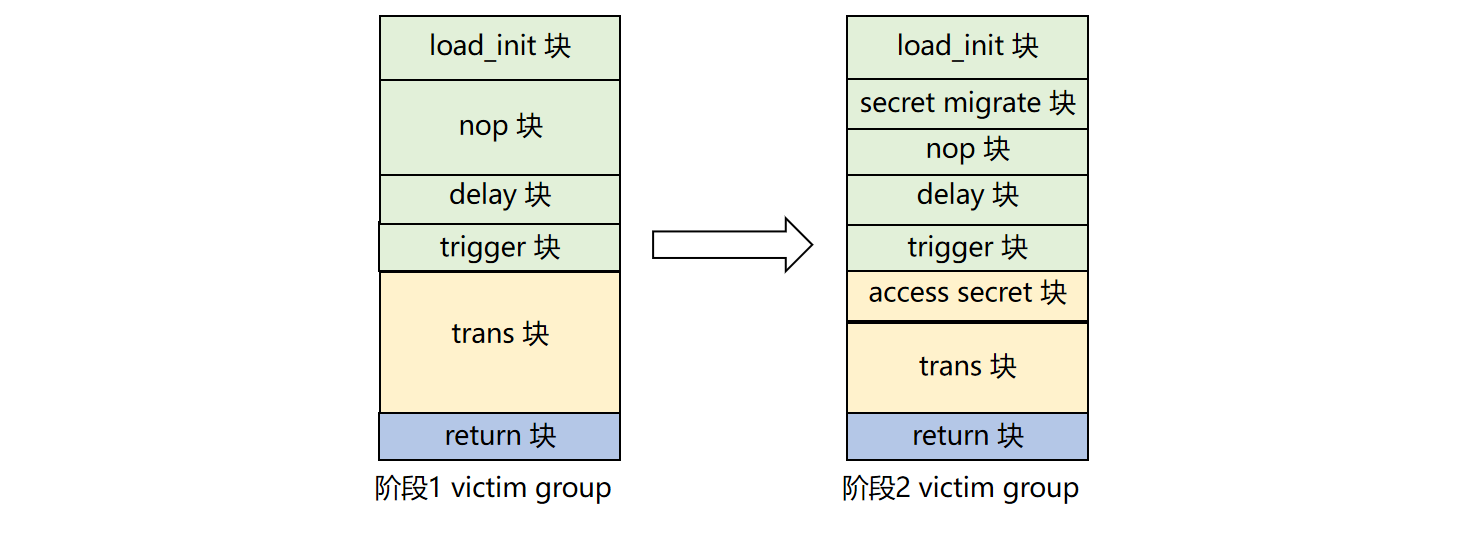
\includegraphics[width=\linewidth]{figure/paper/stage2-access-secret.png}
    \caption{访问秘密数据代码的排布}
    \label{paper:access-secret}
\end{figure}

\subsubsection{侧信道泄露代码的生成与排布}

为了实现侧信道泄露秘密数据的目的,生成框架会生成如下的代码块:\par

\textbf{编码块(encode 块):}
encode 块尝试利用 access\_secret 块访问得到 secret 数据修改处理器的微架构状态,
以此实现将 secret 数据编码到处理器微架构状态的目的。为了让 encode 块有较强的 secret 数据传播和编码能力,
生成的指令会尽可能多的使用 secret 数据,指令间有较强的数据竞争和结构竞争。\par

\textbf{解码块(decode 块):}
decode 块尝试利用 encode 产生的微架构状态差异产生执行时间上的差异,
以此实现将 secret 在处理器微架构的编码利用时间侧信道解码的目的。
因为重复执行相同的指令会涉及到相同微架构部件的使用,从而当一条指令被第二次执行时,
它的执行结果比较容易受到第一次执行时产生的微架构状态的影响,
因此生成框架简单使用和 encode 块相似的代码作为 decode 块。\par

\textbf{秘密数据获得块(get\_secret 块):}
get\_secret 块直接用立即数指令生成 secret 数据的值,并将值存储到和 access\_secret 一致的目的寄存器中。
执行 get\_secret 块可以得到和 access\_secret 块一样的执行结果,但是并不会修改 cache、内存等存储单元。

在进行代码排布时,encode 块需要在瞬态窗口中执行,因此被放置在 trans 块内部,且在 access\_secret 块执行完毕后执行;
decode 块为了可以和 encode 块使用尽可能一样的处理器部件,因此它除了指令和 encode 块高度相似外,
还需要地址和 encode 块保持一致,因此生成框架新定义一个 decode group,
将 decode 块排布在 decode group 中与 encode 块相同的物理地址。\par

decode group 在 victim group 之后执行,用于对 encode 块编码在处理器中的 secret 数据进行解码。
如图\ref{paper:group-switch-all}所示,完整程序在执行时首先执行 train group 序列进行 trigger 指令的训练,
然后切换到 victim group 触发瞬态窗口、访问秘密数据和将秘密数据编码到微架构状态,最后切换到 decode group,
尝试从微架构状态中解码 secret 的值。为了确保 decode group 执行 decode 块时可以获得和 encode 块执行时一样的操作数,从而使用一样的处理器部件,
decode group 复制 victim group 的 load\_init 块、delay 块;trigger 块和 secret\_migration 块用 nop 块替代;
access\_secret 块用 get\_secret 块代替,避免修改cache、内存的状态;decode 块替代 encode 块。
因此 decode group 最后的代码块排布如图\ref{paper:group-switch-all}中的 decode group 所示。\par

\begin{figure}[!h]
    \centering
    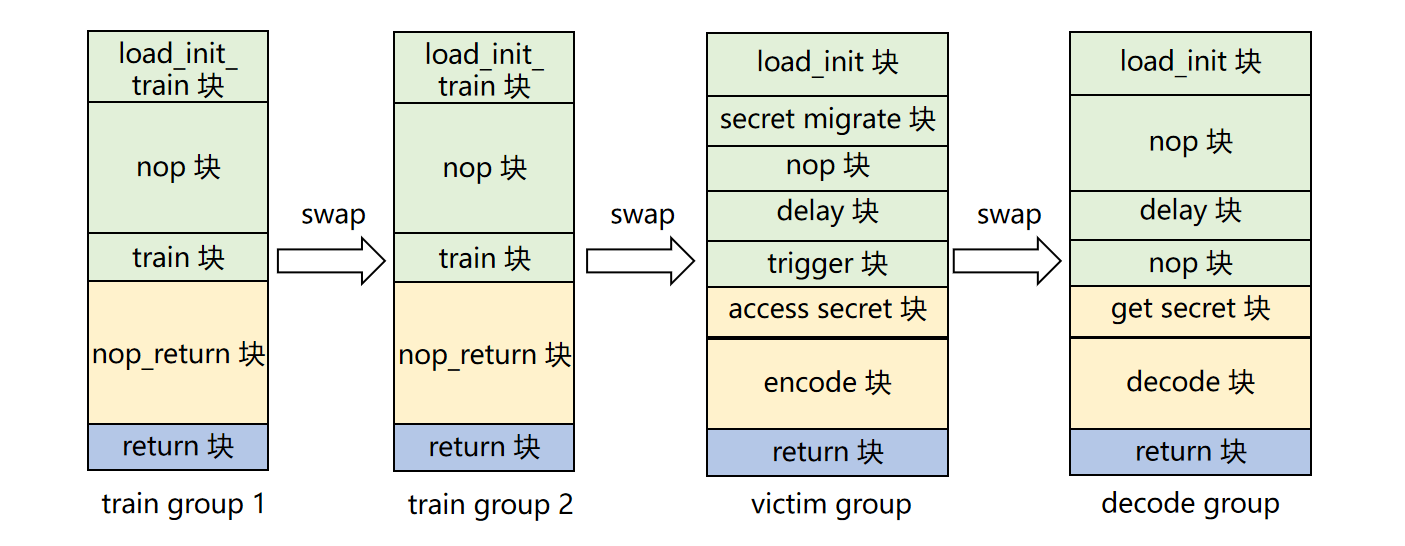
\includegraphics[width=\linewidth]{figure/paper/group-switch-all.png}
    \caption{完整程序内存切换}
    \label{paper:group-switch-all}
\end{figure}

\subsubsection{秘密数据泄露检验}

我们采用差分测试的方法对测试程序是否发生瞬态执行漏洞攻击进行检验。
首先将上述的所有 group 和其他框架代码导出为完整的测试程序,在处理器 RTL 上模拟执行。
为了测量测试程序的执行时间,生成框架会在程序结尾插入特殊 label 指令,
然后对 RTL 进行内部插桩,当该 label 指令被执行时 dump 此时的处理器周期数。
之后将测试程序的 secret 部分替换掉,再次进行模拟执行和 dump 执行结束时的处理器周期数。
如果两者的执行时间存在差异就说明 secret 信息通过时间侧信道泄露出来了,瞬态执行攻击成功,得到完整 PoC。

\section{测试程序生成框架的实现}

本工作由瞬态漏洞测试程序生成框架和硬件处理器插桩修改两部分组成。
其中测试程序生成框架包括 5.2 K 行 Python 和 300 行 riscv 汇编,负责瞬态漏洞测试程序的生成、测试调用和化简;
硬件处理器插桩和修改在开源 riscv 处理器测试框架 starship\cite{starship} 的基础上进行修改,
包括 650 行 C 代码、200 行 Verilog、50 行 chisel,用于提供硬件插桩和测试功能扩展。
我们的测试程序生成框架可以支持 U、S、M 三特权级的测试程序生成,可以支持虚拟地址、物理地址的测试程序生成,
在指令生成方面支持 RISCV 的 rv64imafdc\_zicsr 基本指令扩展,可以高效生成 spectre、meltdown 等典型的瞬态漏洞测试程序。\par

\subsection{硬件插桩和功能扩展}

为了让被测试的处理器满足瞬态漏洞测试程序执行和测试的需要,我们需要对被测试的处理器硬件进行插桩和功能扩展,包括:
a)提供事件监控的软件 label 指令插桩和硬件 rob 插桩;b)提供处理器停机、结束测试程序的软件接口;
c)提供支持物理内存切换的功能的内存模块和触发物理内存切换的软件接口。\par

我们在开源的 riscv 计算机系统评估框架 starship 的基础上进行处理器硬件的修改和测试。
starship 通过继承一系列开源的 riscv 软硬件工具,实现自动化的全栈计算机系统生成,
可以支持 rocket、BOOM、CVA6 等开源 riscv 处理器的仿真、评估、FPGA执行等。
本工作目前仅在 starship 提供的 BOOM flow 的基础上进行测试和评估,
故而下文的硬件插桩和处理器测试仅针对 BOOM 处理器而言。\par

\subsubsection{事件监控和 rob 插桩}
\textbf{label 指令:}
为了了解测试程序在处理器内部的执行情况,检查特殊事件(如瞬态窗口触发、程序执行完毕等)是否被触发,
我们预留了一组 slti 指令作为特殊的 label 指令,并将它们排布在软件的合适位置作为软件插桩。
该部分指令如果被处理器执行,则意味着特殊事件发生。
所有的 label 指令表示的事件、排布的位置等如表\ref{table:label-inst}所示,
因此在生成各个代码块和将它们组织为 group 的时候需要在指定位置额外插入这些 label 指令。\par

\begin{table}[h!]
    \begin{center} 
    \caption{label指令} 
    \label{table:label-inst}  
    \resizebox{1.0\linewidth}{!}{
        \begin{tabular}{|l|l|l|l|} 
            \hline
            \textbf{label名称} & \textbf{汇编指令} & \textbf{排布位置} & \textbf{表示事件}\\
            \hline
            INFO\_VCTM\_START  &  slti zero, zero, 0  & group代码块的第一条代码  & group 开始执行            \\
            INFO\_VCTM\_END    &  slti zero, zero, 1  & group代码块的出口位置    & group 执行完毕            \\
            INFO\_DELAY\_START &  slti zero, zero, 2  & delay块的第一条代码      & 开始数据流延迟执行        \\
            INFO\_DELAY\_END   &  slti zero, zero, 3  & delay块的最后一条代码    & 瞬态窗口关闭              \\
            INFO\_TEXE\_START  &  slti zero, zero, 4  & encode块的第一条代码     & 瞬态窗口触发打开          \\
            INFO\_TEXE\_END    &  slti zero, zero, 5  & encode块的最后一条代码   &                          \\
            INFO\_LEAK\_START  &  slti zero, zero, 6  & decode块的第一条代码     & 开始进行秘密数据泄露       \\
            INFO\_LEAK\_END    &  slti zero, zero, 7  & decode块的最后一条代码   & 秘密数据泄露完毕           \\
            INFO\_INIT\_START  &  slti zero, zero, 8  & init块的第一条代码       & 开始寄存器初始化           \\
            INFO\_INIT\_END    &  slti zero, zero, 9  & init块的最后一条代码     & 寄存器初始化完毕           \\
            INFO\_BIM\_START   &  slti zero, zero, 10 & init\_bim块的第一条代码   & 开始等待 BIM 部件初始化   \\
            INFO\_BIM\_END     &  slti zero, zero, 11 & init\_bim块的最后一条代码 & BIM 部件初始化完毕        \\
            \hline
        \end{tabular}
    }
    \end{center}
\end{table}

\textbf{rob 插桩:}
我们需要对被测试处理器的 ROB 进行硬件插桩,通过监视测试程序中的 label 指令是否进入 rob 和
是否在 rob 中被提交或者回滚,判断瞬态窗口触发、瞬态窗口关闭、程序执行结束等事件是否发生,并记录这些事件发生的时间。
其中瞬态窗口触发事件的发生被用于阶段1的判断,程序执行结束的时间被用于阶段2差分测试的判断。
12 种 label 指令分别代表一类事件,根据 label 是进入 rob 还是从 rob 中提交可以分为 ENQ 和 DEQ 两种子事件,所以一共有 24 种事件。\par

这部分 rob 插桩和事件 log 记录的代码位于 asis/sim/robprofile.v 和 asic/sim/variant/rob\_sync.boom.v 中。
该部分代码首先创建一个 taint.log 文件,然后将监控到的事件信息 dump 到这个 log 文件中,
最后实例化两个 event\_handler 函数调用对 rob 的进入和提交进行周期性检测,
一个负责根据进入 rob 的指令类型记录 ENQ 事件发生;一个负责根据 rob 提交的指令类型记录 DEQ 事件发生。
\begin{figure}[htbp]
    \centering
    \begin{minted}{Verilog}

    initial begin
        $timeformat(-9, 0, "", 20);
        $value$plusargs("taintlog=%s", taintlog);
        event_fd = $fopen({`TOP_DIR, "/wave/", taintlog, ".taint.log"}, "w");
    end

    always @(posedge clock) begin
        if (!reset) begin
            event_handler(`DUT_ROB_ENQ_EN_0, `DUT_ROB_ENQ_INST_0, "ENQ", 0, `IS_DUT);
            event_handler(`DUT_ROB_DEQ_EN_0, `DUT_ROB_DEQ_INST_0, "DEQ", 0, `IS_DUT);
        end
    end

    \end{minted}
    \caption{rob插桩}
    \label{code:rob-stub}
\end{figure}

核心函数 event\_handler 如图\ref{code:event-handler}所示,定义在 rob\_profile.v 中。
该函数记录 rob 检测到的事件,它接收五个参数,其中 valid 表示当前指令进入或者离开 rob,
inst 为当前指令的编码,suffix 为当前指令的子事件类别(ENQ 表示进入 rob、DEQ 表示从 rob 中提交)。
当 valid=1 时,event\_handler 函数根据 inst 和 suffix 的内容选择讲不同的事件 log 信息保存到 taint.log 文件中,
包括事件的名称(如 TEXE\_START\_ENQ、TEXE\_END\_DEQ)和当前的处理器 cycle 数。

\begin{figure}[htbp]
    \centering
    \begin{minted}{Verilog}

    function void event_handler;
        input valid;
        input [31:0] inst;
        input string suffix;
        input int id;
        input int is_dut;

        if (valid) begin
            case (inst)
                `INFO_VCTM_START: $fwrite(event_fd, "%t, VCTM_START_%s, %d, %d\n", $time, suffix, id, is_dut);
                `INFO_VCTM_END: $fwrite(event_fd, "%t, VCTM_END_%s, %d, %d\n", $time, suffix, id, is_dut);
                ...
            endcase
        end
    endfunction
    \end{minted}
    \caption{event\_handler函数}
    \label{code:event-handler}
\end{figure}

\subsubsection{程序退出和打印}
为了在测试程序执行完毕后,结束处理器的运行,退出仿真,我们需要为处理器增加终止仿真执行的软件接口;
此外为了方便对程序的调试,我们需要为处理器增加打印的软件接口。\par

这里我们为处理器扩展了一个用户态只写特权寄存器 probebuffer。该模块定义在 asic/sim/probebuffer.v 文件中,
内部的操作由 dpi-c 接口调用 asic/sim/probebuffer.cpp 中的 parafuzz\_probebuff\_tick 实现,
该函数会根据写入寄存器的值执行退出和打印操作。
为了将 probebuffer 集成到 BOOM 处理器中,我们为 BOOM 的chisel 工程提供了 BlackBox 的 verilog 接口,
并为 probebuffer 分配了 0x800 的 CSR 号。当 csrw 指令写 0x800 特权寄存器时即可调用 probebuffer 的打印和退出程序接口。
接口的具体调用细节如下表。\par

\begin{table}[h!]
    \begin{center} 
    \caption{probebuffer 软件接口} 
    \label{table:probebuffer}  
    \resizebox{0.8\linewidth}{!}{
        \begin{tabular}{|l|l|} 
            \hline
            \textbf{输入} & \textbf{功能}\\
            \hline
            0xAF1B608E883A0000 & probebuff切换到默认工作状态 \\
            0xAF1B608E883A0001 & probebuff切换到打印整数状态 \\
            0xAF1B608E883A0002 & probebuff切换到打印字符状态 \\
            0xAF1B608E883A0003 & probebuff切换到打印地址状态 \\
            0xAF1B608E883B0000 & probebuff执行 exit 函数结束仿真进程 \\
            其他                  & 根据当前工作模式调用 printf 函数输出写入数据 \\
            \hline
        \end{tabular}
    }
    \end{center}
\end{table}

\subsubsection{内存切换和管理}
为了提高 train 块训练 trigger 指令的效果,也为了提高 decode 块对 encode 块编码的解码效果,
程序执行时需要这些指令可以在相同的地址上被执行,因此需要有软硬件机制实现物理内存的指令切换,
根据设计部分的介绍可以知道,这里的物理地址切换是以 group 为单位进行的。
纯软件的物理地址切换可以考虑在执行下一个 group 之前拷贝它的 group 代码覆盖上一个 group 的代码,
这样虽然确保 group 使用同样的物理地址,但是拷贝本身的 overhead 较大,
且严重影响数据 cache 的布局,并且还要解决 icache 的同步问题,
使用效果并不理想;此外也可以通过修改修改页表让不同的 group 共用相同的逻辑地址,但是无法用于物理地址模式下的内存切换。
因此本工作选择直接改写了处理器的 memory 单元,并暴露软件接口来进行物理内存的直接切换,
这样切换的效率最高,对 icache、dcache 的影响最小。\par

\textbf{内存初始化配置}
为了便于改写后的内存单元对内存进行管理和切换,生成框架在生成二进制程序的同时,还会生成一个 libconfig 格式的 config 文件,
用于指示内存单元如何进行内存初始化。config 文件的格式如图\ref{code:memory-config}所示。\par

\begin{figure}[htbp]
    \centering
    \begin{minted}{json}
        start_addr = 2147483648L;
        max_mem_size = 262144;
        memory_regions = (
            {
                type = "dut";
                start_addr = 2147483648L;
                max_len = 61440;
                init_file = "origin_common.bin";
                swap_id = 0;
            },
            ...
            {
                type = "swap";
                start_addr = 2147614720L;
                max_len = 4096;
                init_file = "text_swap_0.bin";
                swap_id = 0;
            }
        );
        swap_list = [1, 0];
    \end{minted}
    \caption{memory config}
    \label{code:memory-config}
\end{figure}

config 的 start\_addr 和 memory\_region 字段表示所需内存的起始地址和长度,内存单元在初始化时会根据这两个字段产生对应大小的内存区域。
memory\_regions 序列表示了需要被内存单元载入的内存块序列的具体信息。start\_addr 表示该内存块的起始地址,max\_len 表示该内存块需要的内存范围,
init\_file 为该内存块指令或者数据所在的 binary 文件的路径。type 表示内存块的种类,如果是 dut 表示这是一个普通的内存块,
程序的框架代码例如 trap 块、init 块、数据部分等不会被切换的内存区域就会被设置为 dut 类型。
内存单元为这个内存块分配 start\_addr-start\_addr+max\_len 的内存范围,然后读取 init\_file 中的二进制内容作为这部分内存的值,
域。\par

如果 type 的类型是 swap,则说明这些内存区域是会被切换的,train group、victim group、decode group 因为会被切换地址范围,
所以被设置为 swap 类型,我们称这部分 memory 为 swap mem\_region。
swap mem\_region 的数据不会被直接初始化到内存单元中,而是会额外分配一块处理器不可达的内存空间 swap mem\_region array 
暂时存放这些内存区域的内容,等需要切换这块内存区域的时候,再将 swap mem\_region array 中的内存区域替换到内存单元中。
为了便于 swap mem\_region 的切换和管理,config 的 memory\_region 结构还包含一个 swap\_id 字段,为每个 swap mem\_region
提供了唯一的 swap 编号(这个编号对于 dut 类型的内存区域没有意义),并维护了一个 swap\_list 的数组。
当处理器执行内存切换的时候,内存单元将按照 swap\_list 中的 swap\_id 依次切换为对应的内存。\par 

在本工作的场景下,所有的 swap mem\_region 共用同一个物理内存地址范围,所以需要额外确保所有的 swap mem\_region 的 start\_addr
和 max\_len 保持一致。\par